\documentclass[12pt]{article}
\usepackage{graphicx}
\graphicspath{ {./images/} }

\title{Coca-Cola Stock Forecasting using ARMA Model}

\author{Zach Joachim, Taylor Jones, Trevor Wai, Carson Watkin}

\begin{document}

\maketitle

\begin{abstract}
 The goal of this paper is to build a model to forcast stock prices and profits of the Coco-Cola Company. Using an Autoregressive Integrated Moving Average (ARIMA) model to create this forcast. Stock prices tend to follow trends during certain periods of time. We attempt to use this data to demonstrate that this data can be used to create reasonable predictions of the behavior of stock prices.\dots
 \end{abstract}

\section{Problem Statement and Motivation}

Stock forecasting is vital for a company that wants to be successfull and profitable. It helps companies 
with financial planning, allowing companies to allocate resources efficiently and make imformed decisions 
about investments and expenditures. It allows companies to identify and mitigate risks associated with a 
volitile market. Finally, along with many other things, forecasting provides a benchmark for the company's 
actual performance to be measured against. By comparing the forecasted stock prices with the actual prices, 
companies can evaluate the effectiveness of their strategies and operations.\par
Clearly the ability to forecast stock prices and other important quantities is of great use and interest to 
companies everywhere.

\section{Data}

The Coca-Cola stock price history data came from a dataset on Kaggle's website. The dataset contains 7 quantities 
indexed by the day of those quantities. These values are the stock's opening price, highesst price point in the day, 
lowest price point in the day, the closing price of the stock, the volume, dividends, and stock slpits of the 
stock for the day. Finding data like this was difficult to find for quantites like profits, margins, or quantities 
for specific drinks that fall under the Coca-Cola umbrella. However, the stock price for a company is a good indicator 
as to what the values are and where they are heading.\par
The stock price data reuqired a little cleaning. For about 50\% the data, the index or date for the stock info 
comes in the form of YYYY-MM-DD, while the other 50\% has the time next to the date, in the same format, 
YYYY-MM-DD HH:MM:SS-UTC\@. For the purposes of our analysis, we only needed the date, and the format it was in was acceptable, 
so what we needed to do was delete part of the index that gave the time. To do this, we stripped the index 
into its list of strings and only kept the part that gave the date, we made this into a new column called \texttt{df['date']}, 
and deleted the original column.

\section{Results}

\subsection{ARIMA Forecast}

We wanted to see if an ARIMA model could accurately predict the next year (365 days) into the future. 
Due to the complexity of the Stock Market and the different parameters of a stock, such as its value 
at Open, Close, Daily High, Daily Low, and the Volume sold, we decided to just look at the value of 
Coca-Cola stock at Open. Due to the large amount of data from the Coca-Cola stock, we decided to just 
analyze the stock from 2009 to 2019 and then forecast into 2020.\par

Like most stocks, the Coca-Cola stock has a lot of noise. To try and compensate for this, we decided 
to take the rolling average over 50 and 200 days to get a smoother trendline. We then perform time series 
forecasting using the ARIMA model on the 50 day rolling average. After splitting our data, we then use the 
\texttt{auto\_arima} class from the \texttt{pmdarima} python package. This allowed us to find the best parameters 
for the ARIMA model based on the training data. The best parameters are then used to train an ARIMA model on the 
dataset. After training the model, we then forecast the next year into the future. The resulting plot shows the historical 
data, the true future data, and the forecasted stock prices.\par

Here we see the different ARIMA models that were tested and the best model that was then selected to predict forecasting.

\begin{verbatim}
Performing stepwise search to minimize aic
 ARIMA(2,2,2)(0,0,0)[0] intercept   : AIC=-14614.840, Time=1.17 sec
 ARIMA(0,2,0)(0,0,0)[0] intercept   : AIC=-14614.126, Time=0.51 sec
 ARIMA(1,2,0)(0,0,0)[0] intercept   : AIC=-14619.359, Time=0.34 sec
 ARIMA(0,2,1)(0,0,0)[0] intercept   : AIC=-14619.441, Time=0.35 sec
 ARIMA(0,2,0)(0,0,0)[0]             : AIC=-14616.124, Time=0.24 sec
 ARIMA(1,2,1)(0,0,0)[0] intercept   : AIC=-14617.515, Time=0.66 sec
 ARIMA(0,2,2)(0,0,0)[0] intercept   : AIC=-14617.494, Time=0.61 sec
 ARIMA(1,2,2)(0,0,0)[0] intercept   : AIC=-14615.679, Time=0.87 sec
 ARIMA(0,2,1)(0,0,0)[0]             : AIC=-14621.441, Time=0.44 sec
 ARIMA(1,2,1)(0,0,0)[0]             : AIC=-14619.515, Time=0.41 sec
 ARIMA(0,2,2)(0,0,0)[0]             : AIC=-14619.495, Time=0.39 sec
 ARIMA(1,2,0)(0,0,0)[0]             : AIC=-14621.358, Time=0.12 sec
 ARIMA(1,2,2)(0,0,0)[0]             : AIC=-14617.680, Time=0.37 sec

Best model:  ARIMA(0,2,1)(0,0,0)[0]          
Total fit time: 6.508 seconds
\end{verbatim}

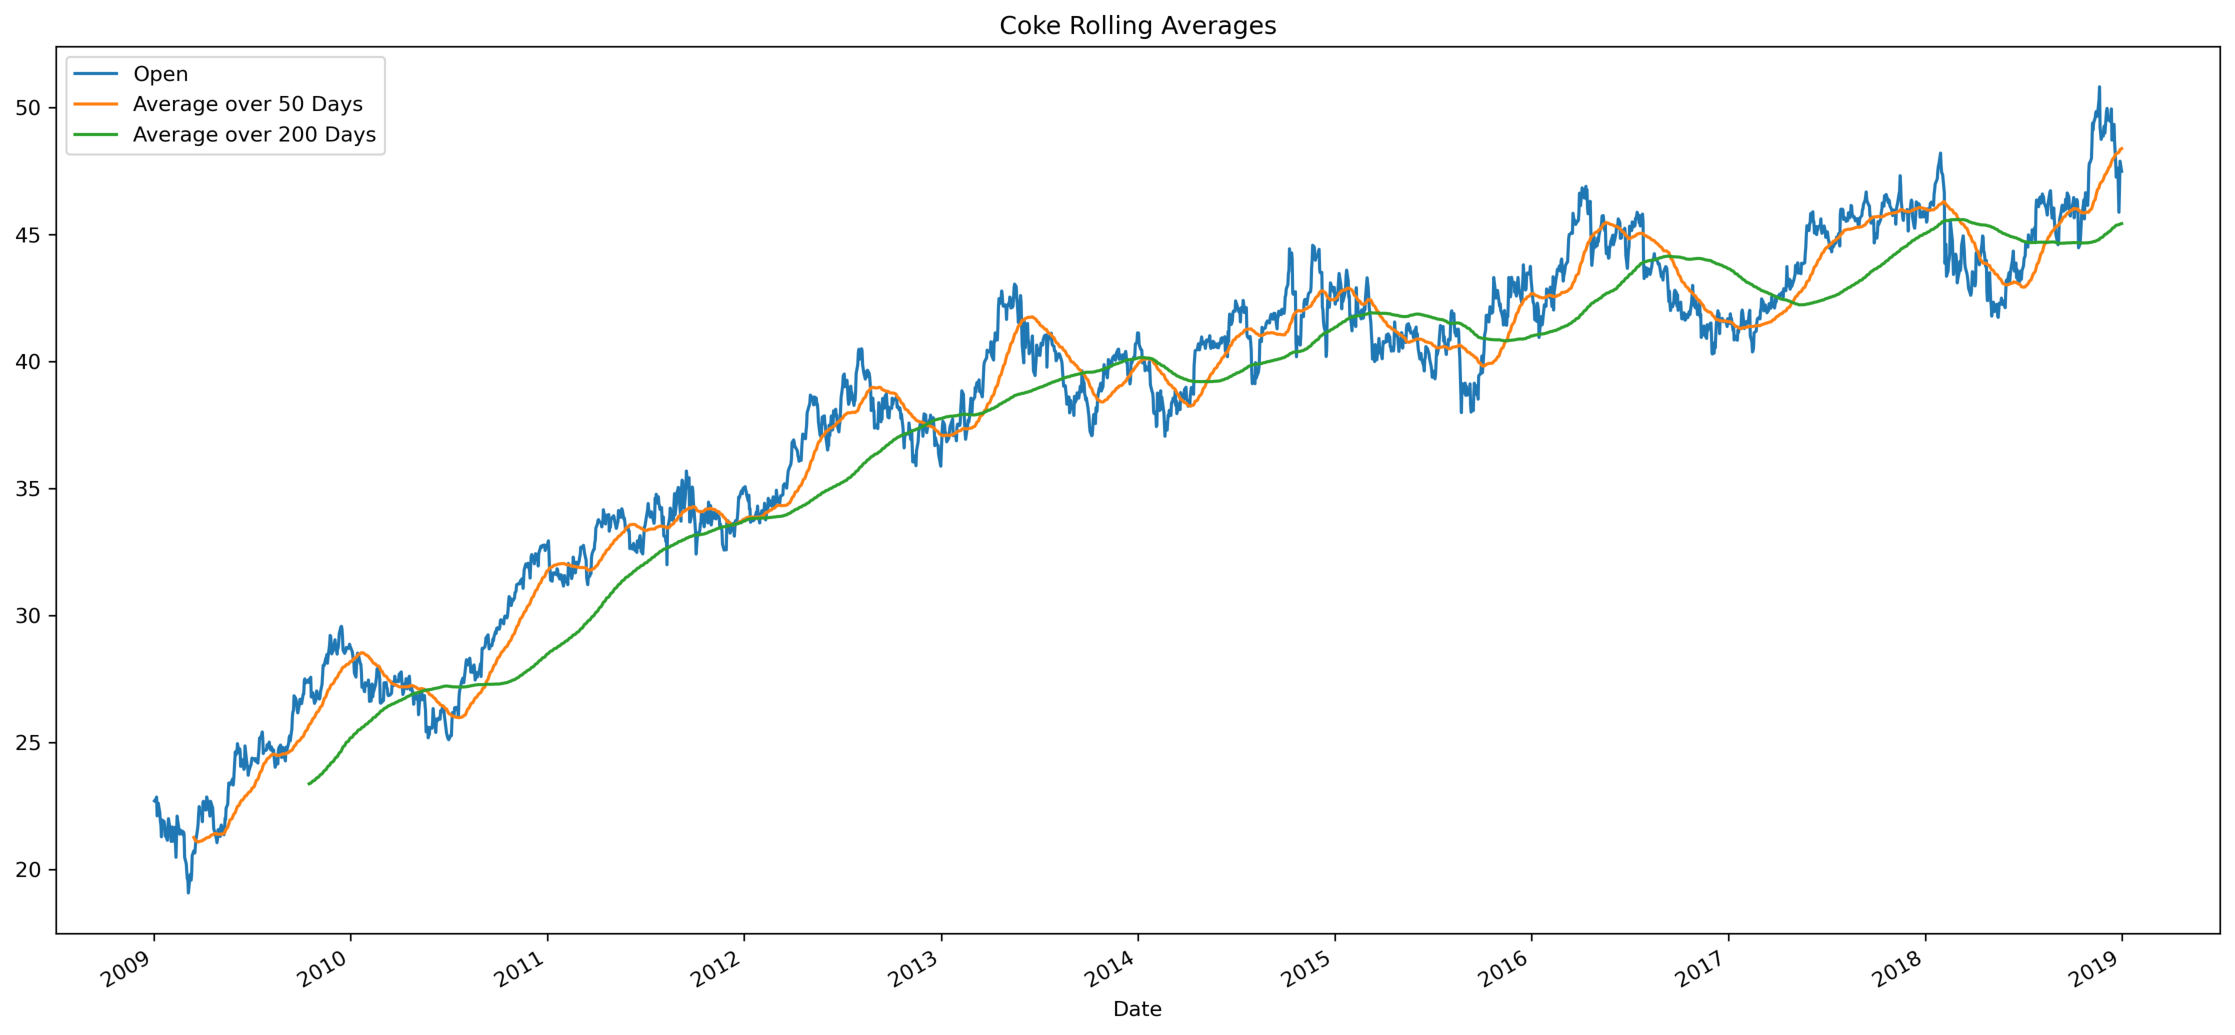
\includegraphics[width=\textwidth]{../images/rolling_average.pdf}

\subsection{Random Forests}
In Random Forest Regression, trees are built randomly, which helps prevent over-fitting. Random Forest Regressors are also well 
suited for noisy data, which is quite typical in stock price data. We trained our model using 100 trees on subsets of our data 
and got an out-of-bag score of 0.9999427215159137, which was surprising given the results of the ARIMA models. After training the 
model, we then predicted the stock price using the whole dataset and got the results shown below:

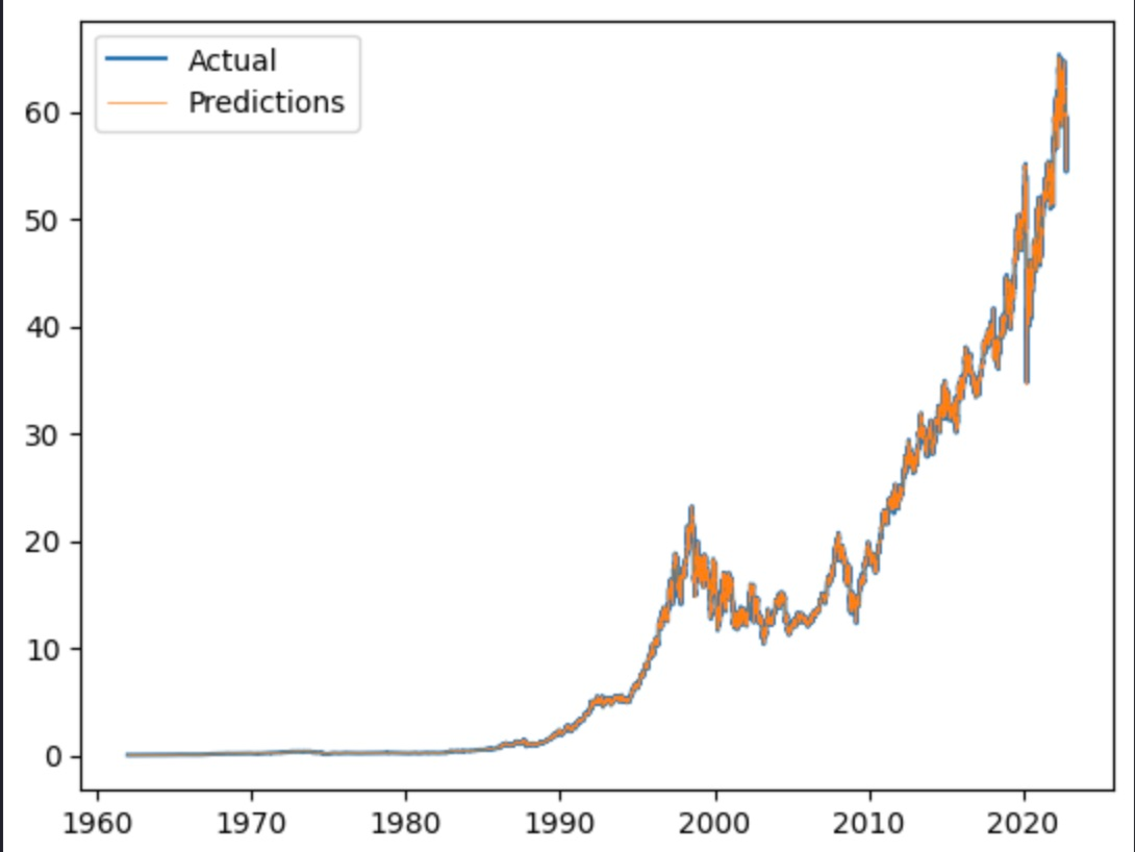
\includegraphics[width=\textwidth]{../images/random_forest_regressor.pdf}


\subsection{Time Series Decomposition of Closing Prices}

Because prices of stocks fluxuate so much we decided to use a seasonal of prices to break down the data. It 
revealed the trend line as well as the seasonal periodic graph as well as the residual noise. We found this to 
be a good method to break down the data because stock prices are slightly periodic through the day and are definetly 
not perfectly linear and so this allowed us to notice trends in our data and see how it changes over time.

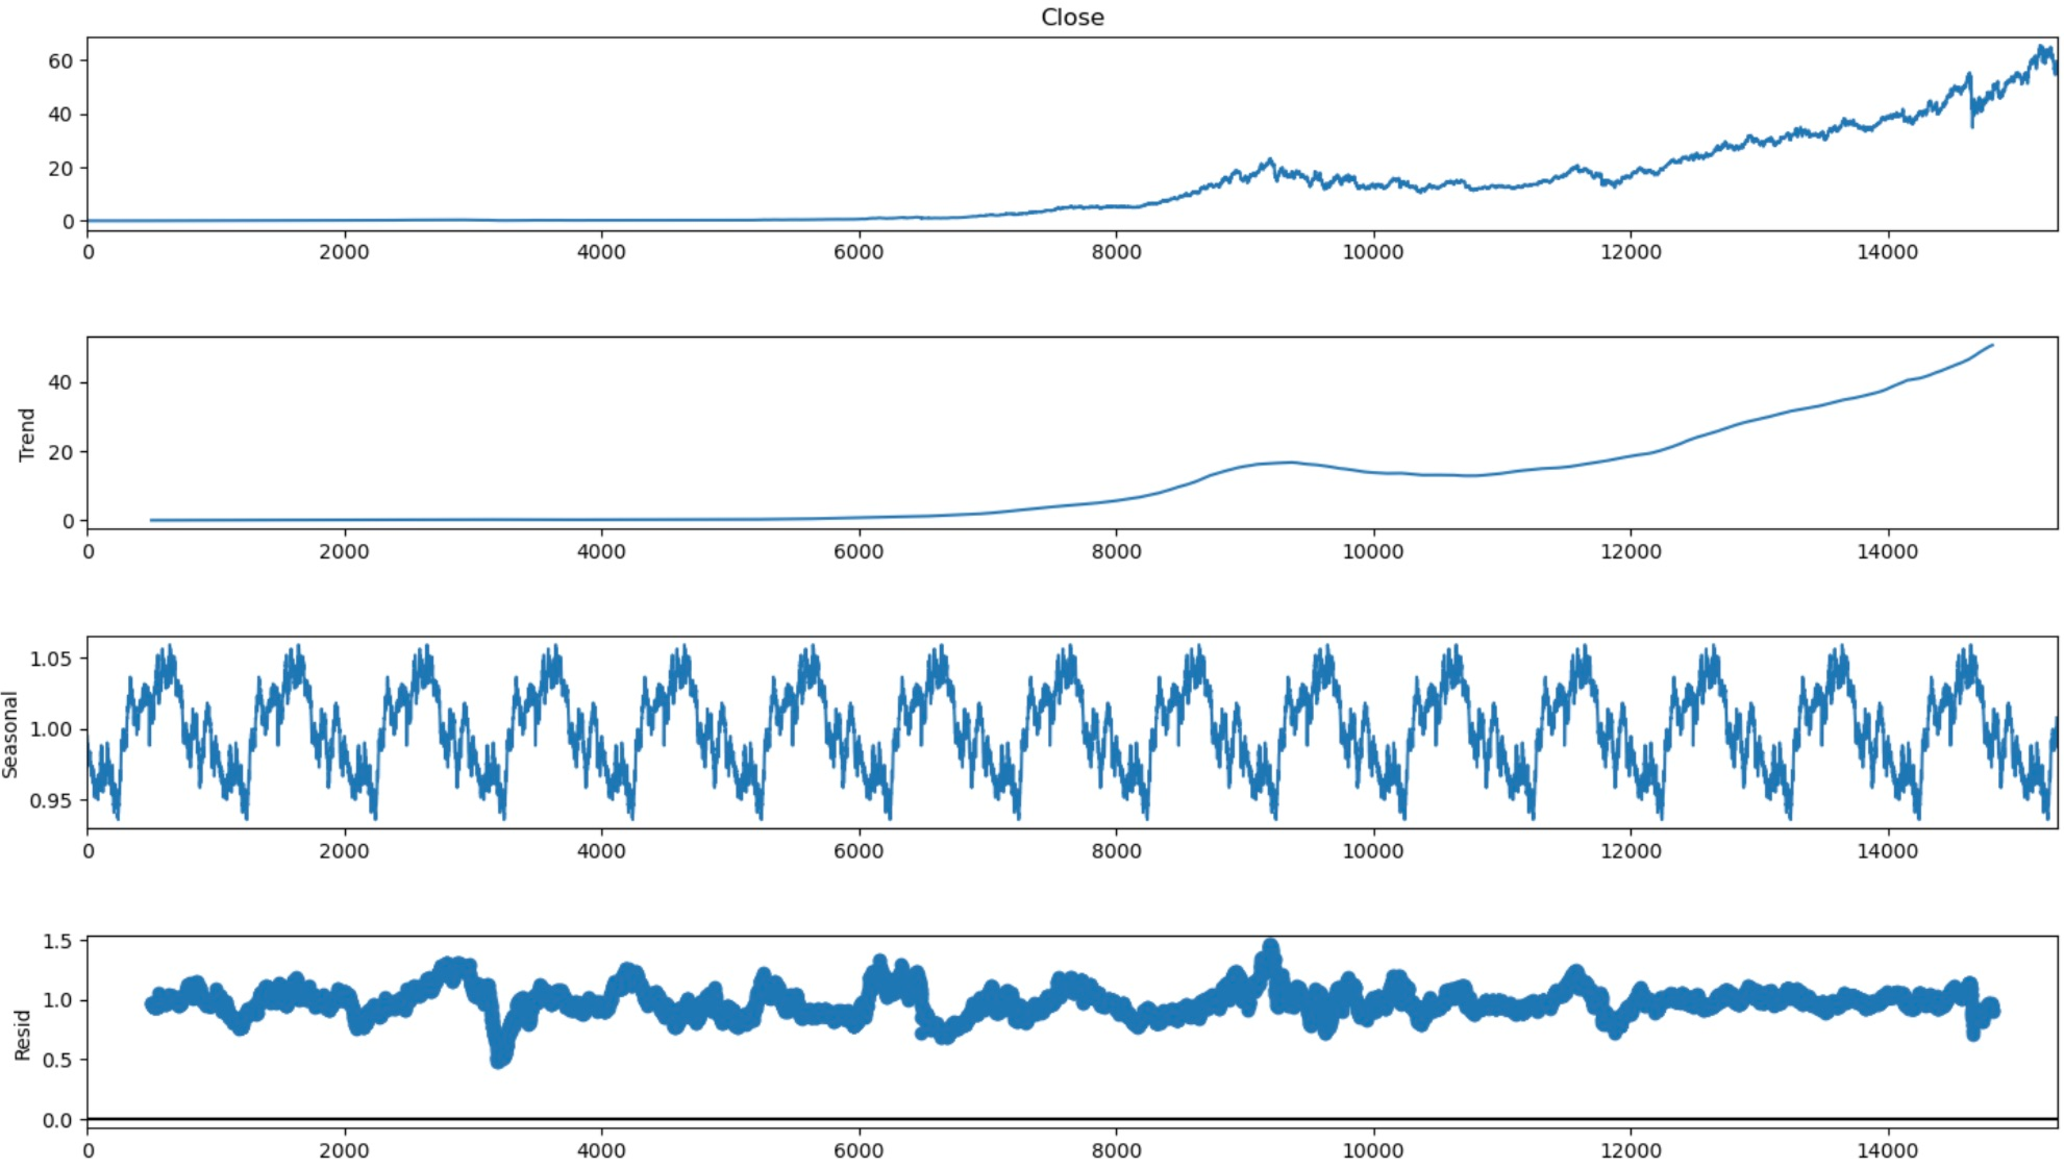
\includegraphics[width=\textwidth]{../images/decomposition.pdf}

\section{Analysis}

\subsection{ARIMA}
Our ARIMA model's performance on the stock price prediction indicates some shortcomings in accuracy. While our ARIMA 
model did predict that the Coca-Cola stock would increase (which overall it did), it failed to show the trends of how 
the stock will drop. It also predicted that the Coca-Cola to be \$63.86 where it should have been at \$53.78. This is 
a \$10.08 difference between the actual cost of Coca-Cola and the forecasted cost. This discrepancy between the 
forecasted and actual values could be attributed to various factors. It's possible that the model failed to capture 
the full complexity of the underlying stock price dynamics, including non-linear trends, seasonality, or sudden shifts 
in market conditions. Additionally, external factors such as unexpected events or changes in economic conditions might 
not have been accounted for in the model, leading to inaccuracies in the predictions. Further analysis, including model 
refinement, incorporating additional data features, or exploring alternative forecasting methods, may be necessary to 
improve the accuracy of future predictions and better capture the dynamic nature of stock price movements.


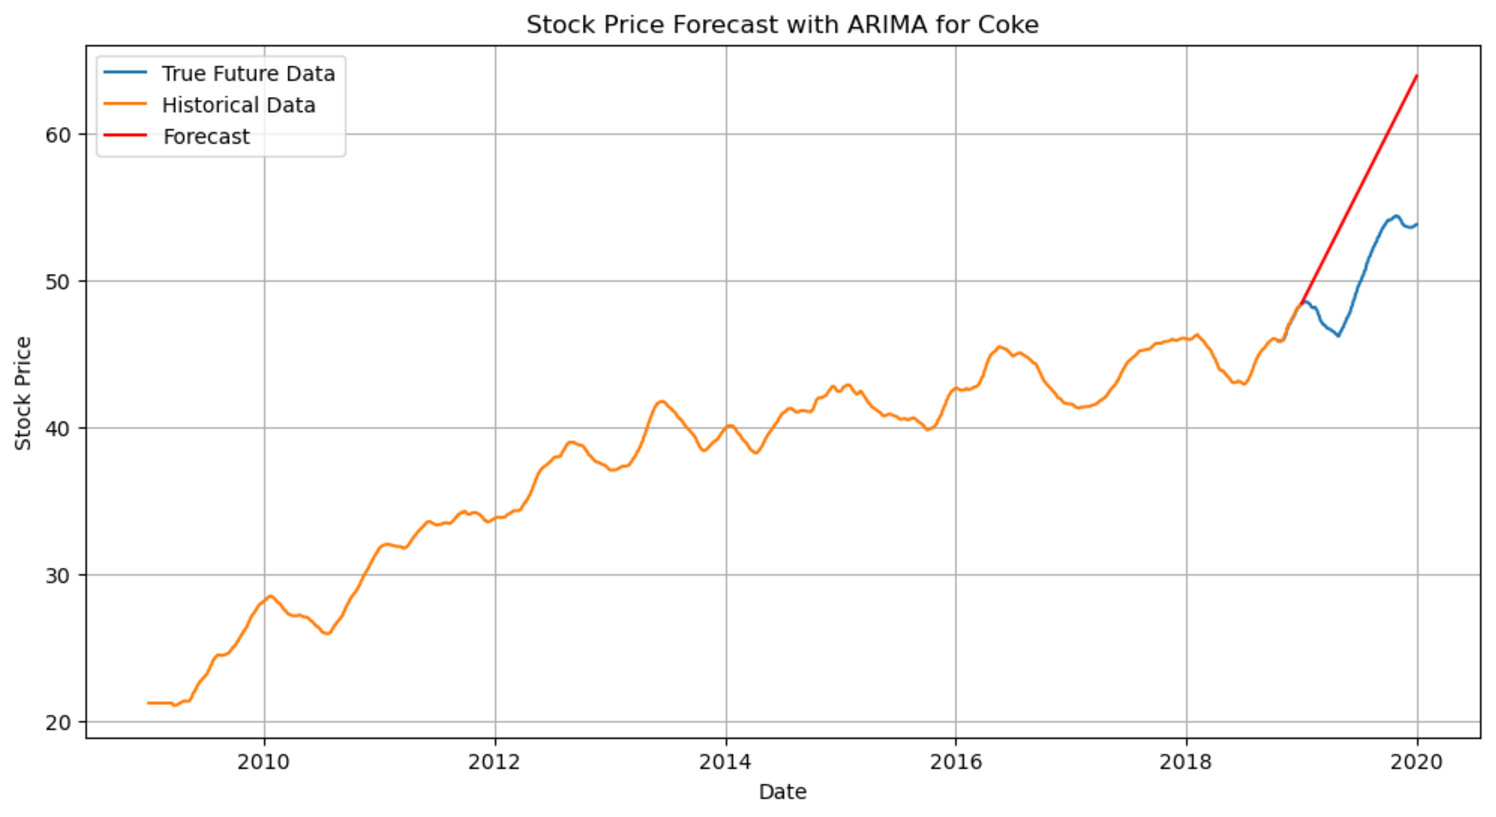
\includegraphics[width=\textwidth]{../images/ARIMA-Coke.pdf}


\subsection{Random Forests}
Random Forest Regressors tend to perform well with noisy data such as ours, however, the model still had 
trouble predicting the larger spikes over time such as that through 1995--2005. Overall, this model performed 
better than the ARIMA model that we suspected would be good for this dataset, we had not thought of the 
impact that the noise in the data would have on the ARIMA model.

\section{Ethical Implications}

The primary ethical concern of our project is the application of our analysis. Individuals wanting to manipulate the stock market would be able to use our model as their evidence to artificially manipulate supply and demand. This interferes with the free and fair operation of the stock market and is illegal in the United States. An example of how manipulators can use our analysis to affect the market is through stock bashing. Our analysis could predict the fall of a stock price and then perpetrators can use this as evidence for stock bashing or convincing the public that a stock price is worth less. Therefore allowing them to purchase the stock at a cheaper price to try and later turn a profit. \par
Therefore we should add a disclaimer in our project that all of the analysis and predictions created are simply models and not prophecies of events to come. Therefore people understand that our analysis is simply trying to predict how the stock prices are going to fluxuate and this can simply be a factor in their buying and selling of shares.
\section{Conclusion}
Overall, the traditional time-series model (ARIMA) that we expected to perform well with our data did not predict the future price of stocks accurately. The predictions seemed to be very sensitive to the behavior just before predicting. This could be due to the volatility of stocks and the lack of a clear period to base our models on.\par
On the other hand, the random forest regressor model tended to perform really well, with error in the estimates being really low. We don't know why this is.
\end{document}